% !TEX root = ../popl-paper.tex

\begin{figure}[t]
	\begin{center}
		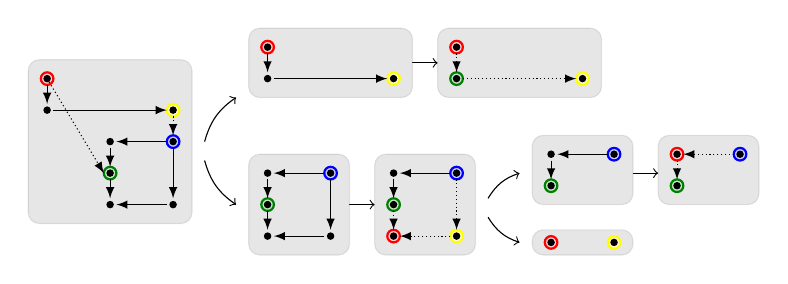
\begin{tikzpicture}[scale = .8]
			\begin{scope}
				\draw[gray,fill = gray, rounded corners, opacity=0.2] (-.3,.3) rectangle (2.3,-2.3);
				\draw[red, thick, fill = red!20] (0,0) circle (0.1);
				\draw[Green, thick, fill = Green!20] (1,-1.5) circle (0.1);
				\draw[Yellow, thick, fill = Yellow!20] (2,-.5) circle (0.1);
				\draw[blue, thick, fill = blue!20] (2,-1) circle (0.1);

				\draw[black, fill = black] (0,0) circle (.05);
				\draw[black, fill = black] (0,-.5) circle (.05);
				\draw[black, fill = black] (2,-.5) circle (.05);
				\draw[black, fill = black] (1,-1) circle (.05);
				\draw[black, fill = black] (2,-1) circle (.05);
				\draw[black, fill = black] (1,-1.5) circle (.05);
				\draw[black, fill = black] (1,-2) circle (.05);
				\draw[black, fill = black] (2,-2) circle (.05);

				\draw[>=latex, ->] (0,-.1) to (0, -.4);
				\draw[>=latex, ->,  densely dotted] (0,0) to (.9, -1.5);
				\draw[>=latex, ->] (.1,-.5) to (1.9, -.5);
				\draw[>=latex, ->,  densely dotted] (2,-.6) to (2, -.9);
				\draw[>=latex, ->] (1.9,-1) to (1.1, -1);
				\draw[>=latex, ->] (1,-1.1) to (1, -1.4);
				\draw[>=latex, ->] (1,-1.6) to (1, -1.9);
				\draw[>=latex, ->] (2,-1.1) to (2, -1.9);
				\draw[>=latex, ->] (1.9,-2) to (1.1, -2);

				\draw[->] (2.5,-1) to[bend left = 20] (3,-.3);
				\draw[->] (2.5,-1.3) to[bend right = 20] (3,-2);
				\draw[->] (7,-1.9) to[bend left = 20] (7.5,-1.5);
				\draw[->] (7,-2.2) to[bend right = 20] (7.5,-2.6);

				\draw[=>latex, ->] (5.8,.25) to (6.2,.25);
				\draw[=>latex, ->] (4.8,-2) to (5.2,-2);
				\draw[=>latex, ->] (9.3,-1.5) to (9.7,-1.5);
			\end{scope}
			\begin{scope}[shift = {(3.5,.5)}]
				\draw[gray,fill = gray, rounded corners, opacity=0.2] (-.3,.3) rectangle (2.3,-.8);
				\draw[red, thick, fill = red!20] (0,0) circle (0.1);
				\draw[Yellow, thick, fill = Yellow!20] (2,-.5) circle (0.1);

				\draw[black, fill = black] (0,0) circle (.05);
				\draw[black, fill = black] (0,-.5) circle (.05);
				\draw[black, fill = black] (2,-.5) circle (.05);

				\draw[>=latex, ->] (0,-.1) to (0, -.4);
				\draw[>=latex, ->] (.1,-.5) to (1.9, -.5);
			\end{scope}
			\begin{scope}[shift = {(6.5,.5)}]
				\draw[gray,fill = gray, rounded corners, opacity=0.2] (-.3,.3) rectangle (2.3,-.8);
				\draw[red, thick, fill = red!20] (0,0) circle (0.1);
				\draw[Green, thick, fill = Green!20] (0,-.5) circle (0.1);
				\draw[Yellow, thick, fill = Yellow!20] (2,-.5) circle (0.1);

				\draw[black, fill = black] (0,0) circle (.05);
				\draw[black, fill = black] (0,-.5) circle (.05);
				\draw[black, fill = black] (2,-.5) circle (.05);

				\draw[>=latex, ->, densely dotted	] (0,-.1) to (0, -.4);
				\draw[>=latex, ->, densely dotted	] (.1,-.5) to (1.9, -.5);
			\end{scope}
			\begin{scope}[shift = {(2.5,-.5)}]
				\draw[gray,fill = gray, rounded corners, opacity=0.2] (.7,-.7) rectangle (2.3,-2.3);
				\draw[Green, thick, fill = Green!20] (1,-1.5) circle (0.1);
				\draw[blue, thick, fill = blue!20] (2,-1) circle (0.1);

				\draw[black, fill = black] (1,-1) circle (.05);
				\draw[black, fill = black] (2,-1) circle (.05);
				\draw[black, fill = black] (1,-1.5) circle (.05);
				\draw[black, fill = black] (1,-2) circle (.05);
				\draw[black, fill = black] (2,-2) circle (.05);
				\draw[>=latex, ->] (1.9,-1) to (1.1, -1);
				\draw[>=latex, ->] (1,-1.1) to (1, -1.4);
				\draw[>=latex, ->] (1,-1.6) to (1, -1.9);
				\draw[>=latex, ->] (2,-1.1) to (2, -1.9);
				\draw[>=latex, ->] (1.9,-2) to (1.1, -2);
			\end{scope}
			\begin{scope}[shift = {(4.5,-.5)}]
				\draw[gray,fill = gray, rounded corners, opacity=0.2] (.7,-.7) rectangle (2.3,-2.3);
				\draw[red, thick, fill = red!20] (1,-2) circle (0.1);
				\draw[Green, thick, fill = Green!20] (1,-1.5) circle (0.1);
				\draw[Yellow, thick, fill = Yellow!20] (2,-2) circle (0.1);
				\draw[blue, thick, fill = blue!20] (2,-1) circle (0.1);

				\draw[black, fill = black] (1,-1) circle (.05);
				\draw[black, fill = black] (2,-1) circle (.05);
				\draw[black, fill = black] (1,-1.5) circle (.05);
				\draw[black, fill = black] (1,-2) circle (.05);
				\draw[black, fill = black] (2,-2) circle (.05);
				\draw[>=latex, ->] (1.9,-1) to (1.1, -1);
				\draw[>=latex, ->] (1,-1.1) to (1, -1.4);
				\draw[>=latex, ->,  densely dotted] (1,-1.6) to (1, -1.9);
				\draw[>=latex, ->,  densely dotted] (2,-1.1) to (2, -1.9);
				\draw[>=latex, ->,  densely dotted] (1.9,-2) to (1.1, -2);
			\end{scope}

			\begin{scope}[shift = {(7,-.5)}]
				\draw[gray,fill = gray, rounded corners, opacity=0.2] (.7,-.4) rectangle (2.3,-1.5);
				\draw[blue, thick, fill = blue!20] (2,-.7) circle (0.1);
				\draw[Green, thick, fill = Green!20] (1,-1.2) circle (0.1);

				\draw[black, fill = black] (1,-.7) circle (.05);
				\draw[black, fill = black] (2,-.7) circle (.05);
				\draw[black, fill = black] (1,-1.2) circle (.05);

				\draw[>=latex, ->] (1.9,-.7) to (1.1, -.7);
				\draw[>=latex, ->] (1,-.8) to (1, -1.1);
			\end{scope}

			\begin{scope}[shift = {(9,-.5)}]
				\draw[gray,fill = gray, rounded corners, opacity=0.2] (.7,-.4) rectangle (2.3,-1.5);
				\draw[red, thick, fill = red!20] (1,-.7) circle (0.1);
				\draw[blue, thick, fill = blue!20] (2,-.7) circle (0.1);
				\draw[Green, thick, fill = Green!20] (1,-1.2) circle (0.1);

				\draw[black, fill = black] (1,-.7) circle (.05);
				\draw[black, fill = black] (2,-.7) circle (.05);
				\draw[black, fill = black] (1,-1.2) circle (.05);

				\draw[>=latex, ->,  densely dotted] (1.9,-.7) to (1.1, -.7);
				\draw[>=latex, ->,  densely dotted] (1,-.8) to (1, -1.1);
			\end{scope}

			\begin{scope}[shift = {(7,-.6)}]
				\draw[gray,fill = gray, rounded corners, opacity=0.2] (.7,-1.8) rectangle (2.3,-2.2);
				\draw[red, thick, fill = red!20] (1,-2) circle (0.1);
				\draw[Yellow, thick, fill = Yellow!20] (2,-2) circle (0.1);

				\draw[black, fill = black] (1,-2) circle (.05);
				\draw[black, fill = black] (2,-2) circle (.05);
			\end{scope}

		\end{tikzpicture}
	\end{center}
  \caption{Decomposition game for the MSC of Fig.~\ref{fig:pp_ex}. This is a 3-winning game for Eve.}
  \label{fig:stw-ex}
\end{figure}
